\section{Results}
\label{sec:results}
This section will present convergence and runtime results of the scheduling algorithm.

\subsection{Energy Convergence}
\label{sec:convergence}
For the pure Python implementation of the MCMC scheduler, we recorded average energy and variance in between sweeps, which are documented in \Cref{fig:convergence-14h} and \Cref{fig:convergence-8h} for different lengths of day. Both figures compare different sweep exponents $q$ from $-1$ to $-3$, which governs how the temperature varies over the course of the simulation, and how that affects the convergence speed.

\begin{figure}[H]
  \centering
  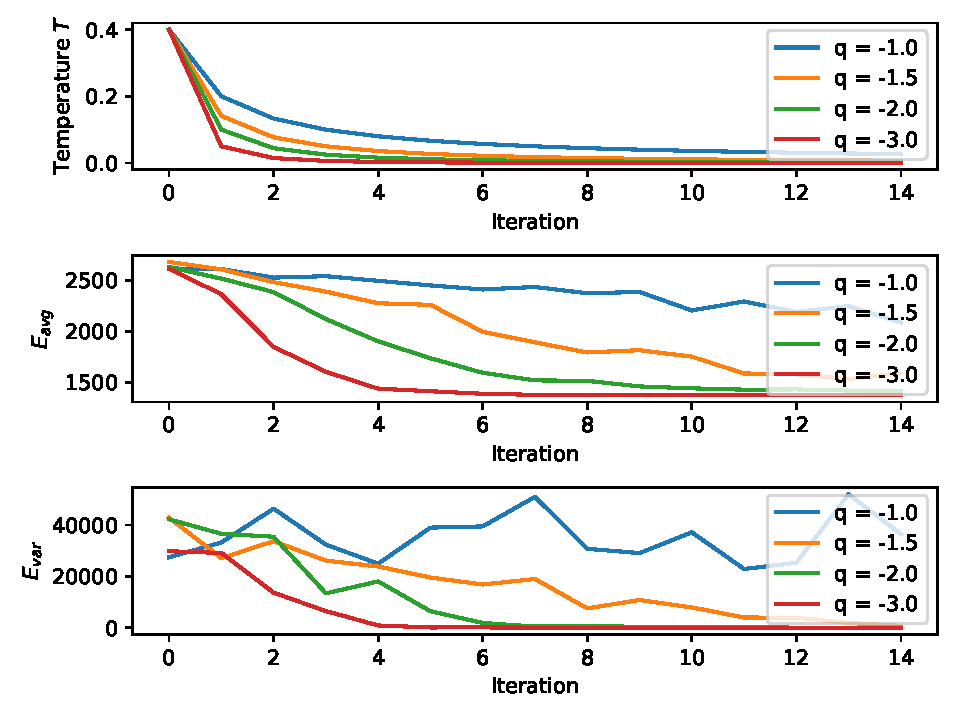
\includegraphics[width=0.8\linewidth]{results/convergence-14h-day.pdf}
  \caption{Temperature, average energy $E_{avg} = \langle E \rangle$ and energy variance $E_{var} = \left\langle\Delta E^2\right\rangle$ for a 14-hour work day. Low variance can be used as a stopping criterion (cf. \Cref{sec:theory}).}
  \label{fig:convergence-14h}
\end{figure}

As we can see, the average energy $\langle E \rangle$ generally decreases, and much faster so for higher values of $|q|$. The variance at the bottom stays high for the slowly-progressing run, indicating that convergence has not yet been achieved, but decays quicker for stronger temperature decreases (in red).

\begin{figure}[H]
  \centering
  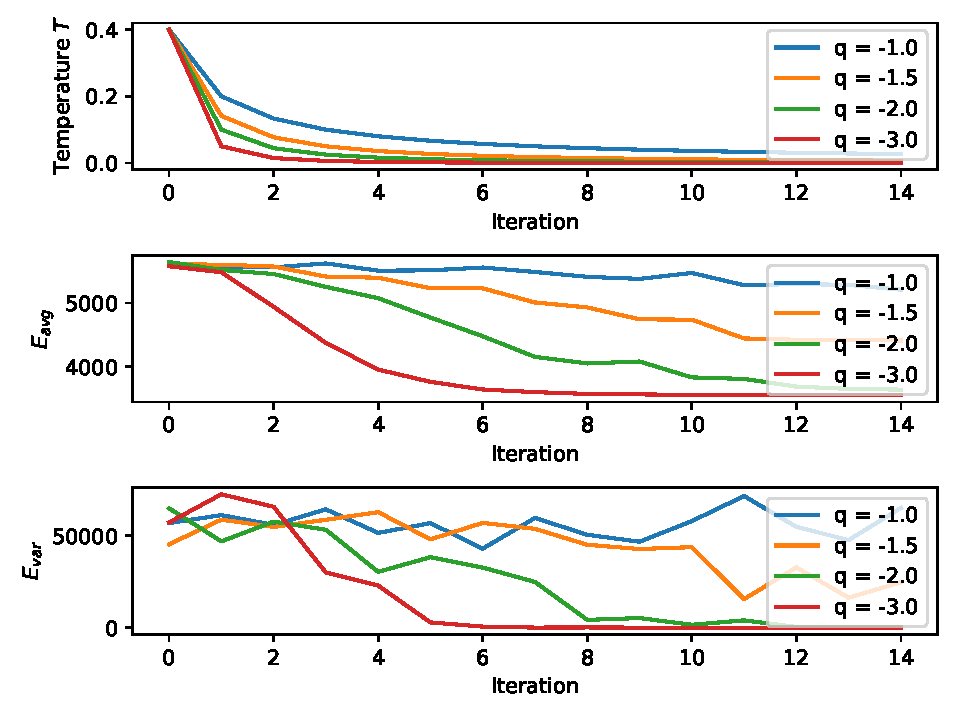
\includegraphics[width=0.8\linewidth]{results/convergence-8h-day.pdf}
  \caption{Temperature, average energy $E_{avg} = \langle E \rangle$ and energy variance $E_{var} = \left\langle\Delta E^2\right\rangle$ for an 8-hour work day. The average energy here is higher than in \Cref{fig:convergence-14h} because days are shorter and therefore long-duration task orderings matter a lot more, negatively impacting the optimality.}
  \label{fig:convergence-8h}
\end{figure}

\subsection{Runtime Performance}
\label{sec:runtime}
The following benchmarks were all accumulated on an x86\_64 Intel\textregistered \, i7-5600U CPU running at \SI{2.6}{\giga\hertz} verified through 3 individual runs, keeping parameters consistent along them.

\Cref{table:profile} contains profiling data of the pure Python implementation.
Considering the high number of calls but low own time per function call, this suggests that there is little progress to be made using only Python, motivating the use of Numba and the low-level implementations in C++ and Rust to compare.

\begin{table}[H]
  \vspace{0.5cm}
  \centering
  \caption{Runtime Comparison of the different implementations run on the same scenarios with $N = 80$ tasks. Each runtime is given as the average over three runs.}
  \begin{tblr}{
    colspec={llr},
    row{2,3} = {bg=azure9},
        row{4} = {bg=violet9},
        row{5} = {bg=cyan9},
      }
    \hline
    \bf Implementation & \bf Language & \bf Runtime / seconds \\
    \hline
    MCMCScheduler      & Python & 31.3887 \\
    NumbaMCMCScheduler & Python & 1.9335 \\
    \hline
    RustyMCMCScheduler & Rust & 0.4034 \\
    \hline
    CppMCMCScheduler   & C++ & 0.4062
    \hline
  \end{tblr}
  \label{table:runtime}
\end{table}

And indeed, \Cref{table:runtime} shows us a 77-times speed up of the Rust and C++ implementations as compared to the pure Python implementation.
\Cref{fig:complexity} reinforces this data for different input sizes, also revealing the complexity proportionality.
As expected, Rust and C++, both compiled languages, perform very similarly in terms of their runtime.
Memory usage analysis was not carried out as part of this project, but we suspect Rust and C++ to perform equivalently once again.

What is perhaps more surprising is that Numba is almost five times slower than the Rust and C++ implementations, which is rooted in the limitations of the just-in-time compilation of Python code.
Nevertheless, Numba achieves an impressive speed-up, being 15 times faster than the pure Python implementation.
One should also note that the Numba compilation time was approximately 3.2 seconds, taking place once for each Python process.

\begin{figure}[H]
  \centering
  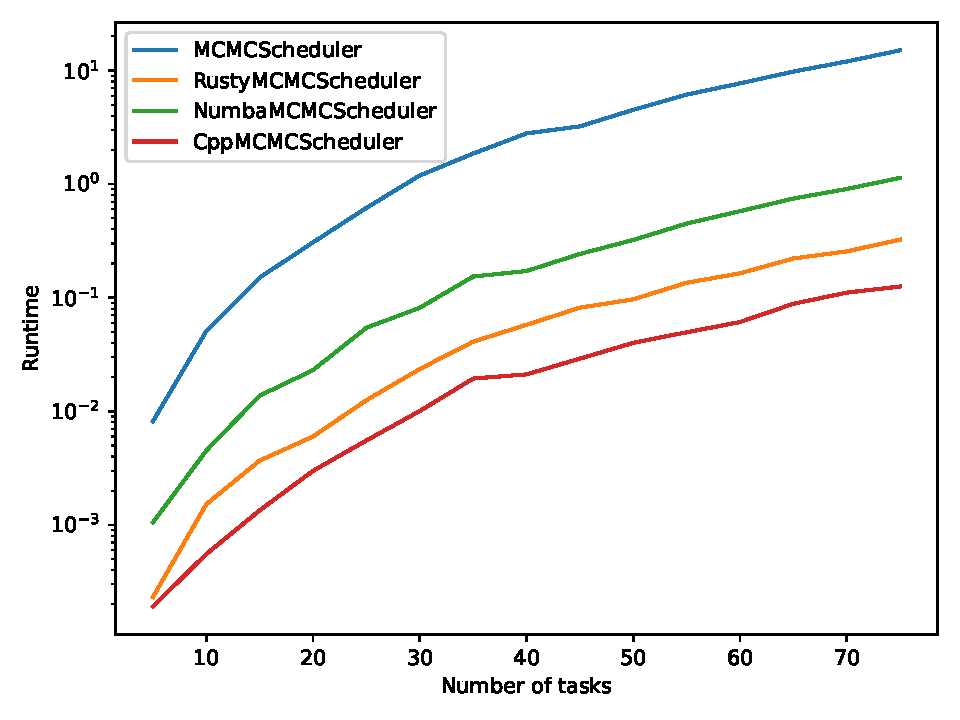
\includegraphics[width=0.68\linewidth]{results/complexity.pdf}
  \caption{The runtimes of each implementation of the scheduler algorithm (Python, Rust, Python Numba, C++) for an increasing number of tasks.}
  \label{fig:complexity}
\end{figure}

Fitting a first-order polynomial on the logarithm of the runtime vs the logarithm of the number of tasks, so through the individual lines in \Cref{fig:complexity}, we obtain the following slopes:

\begin{itemize}
  \tightlist
  \item MCMCScheduler: 2.874
  \item RustyMCMCScheduler: 2.728
  \item NumbaMCMCScheduler: 2.678
  \item CppMCMCScheduler: 2.570
\end{itemize}

So the empirical runtime complexity of the algorithm is between $\mathcal{O}(2.5)$ and $\mathcal{O}(2.9)$.

\begin{table}[H]
  \centering
  \caption{Profile obtained by running \bash{inv profile-scheduler | grep purepython.py}.}
  \begin{tabular}{rrrrrll}
    \hline
    \bf Ncalls & \bf Total & \bf / call & \bf Cum. & \bf / call & \bf Filename:line & \bf Function     \\
    \hline
    1          & 0.000     & 0.000      & 14.236   & 14.236     & purepython:142    & schedule         \\
    10         & 0.209     & 0.021      & 14.235   & 1.424      & purepython:123    & mcmcSweep        \\
    36010      & 1.144     & 0.000      & 13.784   & 0.000      & purepython:97     & computeEnergy    \\
    2196671    & 5.391     & 0.000      & 11.353   & 0.000      & purepython:41     & spreadTasks      \\
    1006332    & 1.389     & 0.000      & 1.842    & 0.000      & purepython:27     & generateNextSlot \\
    2196610    & 0.798     & 0.000      & 0.972    & 0.000      & purepython:108    & <genexpr>        \\
    2196610    & 0.384     & 0.000      & 0.384    & 0.000      & purepython:106    & <genexpr>        \\
    36000      & 0.082     & 0.000      & 0.217    & 0.000      & purepython:83     & permuteState     \\
    36011      & 0.046     & 0.000      & 0.124    & 0.000      & purepython:19     & startingSlot     \\
  \end{tabular}
  \label{table:profile}
\end{table}
